\documentclass[a4paper]{article}
%\usepackage{fourier-otf}
\usepackage[utf8]{inputenc}
\usepackage{graphicx}
\usepackage{algorithm}
\usepackage{algpseudocode}
\usepackage{float}
\usepackage{lipsum}
\usepackage{scrextend}
\usepackage{biblatex}
\addbibresource{bibliography.bib}
\usepackage{listings}
\usepackage{amsmath}
\usepackage{amsfonts}
%\usepackage[square,sort,comma,numbers]{natbib}
\newtheorem{theorem}{Theorem}[section]
\usepackage{color}
\usepackage{makeidx}
\usepackage{titlepic}
\definecolor{mygreen}{rgb}{0,0.6,0}
\definecolor{mygray}{rgb}{0.5,0.5,0.5}
\definecolor{mymauve}{rgb}{0.58,0,0.82}
\lstset{ %
	backgroundcolor=\color{white},   % choose the background color
	basicstyle=\footnotesize,        % size of fonts used for the code
	breaklines=true,                 % automatic line breaking only at whitespace
	captionpos=b,                    % sets the caption-position to bottom
	commentstyle=\color{mygreen},    % comment style
	escapeinside={\%*}{*)},          % if you want to add LaTeX within your code
	keywordstyle=\color{blue},       % keyword style
	stringstyle=\color{mymauve},     % string literal style
}
\usepackage{hyperref}
\hypersetup{
  colorlinks   = true,    % Colours links instead of ugly boxes
  urlcolor     = black,    % Colour for external hyperlinks
  linkcolor    = black,    % Colour of internal links
  citecolor    = black      % Colour of citations
}
%\title{First chapter}

%\author{F.Bernardi}

%\protect\\ 

\newcommand{\myName}{Fabrizio Bernardi}
\newcommand{\myTitle}{Modeling and data analysis of the calcium activity in somatostatin interneurons from in vivo imaging on mice }
\newcommand{\myDegree}{Programme: \protect\\ \textit{Mathematical Engineering}}
\newcommand{\myCycle}{XXXI cycle}
\newcommand{\myDepartment}{Department of Mathematics}
\newcommand{\myUni}{Politecnico di Milano}
\newcommand{\myYear}{2022}
\newcommand{\myTime}{01 Jan \myYear}

\pdfbookmark{Cover}{cover}

\begin{document}
	
	
	
\section{Interbrain data analysis: emotion discrimination task}

In this second chapter, the main results on the data analysis for the emotion discrimination task are presented. After describing the phases of the task and trying to understand which could be an appropriate way  to represent the data through normalizations, first considerations on the neural activity of mice, in relation to their behaviour, are taken into account. Then, the focus goes to the main part of the analysis: the \textit{interbrain synchrony} among neural activities. The different concepts of synchrony introduced in Chapter 2 have been investigated, i.e. the cross-correlation between the mean activities of the mice and the peak synchronization among neurons. Finally, the topic of causality between signal is dealt using the tool of Granger prediction.\\
 All the results refer to two versions of the emotion discrimination task: a standard task, where the observer is in a \textit{neutral condition}, and the \textbf{self-experience task}, in which the observer has been stressed before the task.


\subsection{Emotion discrimination task}

\begin{figure}[H]
	\begin{center}
		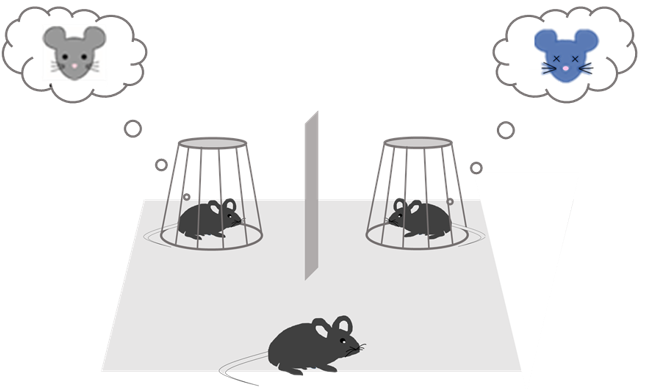
\includegraphics[scale=.90]{emotion_discrimination.png} 
	\end{center} 
	\caption{\textit{Scheme of the emotion discrimination task.}}
	
\end{figure}

In the \textit{emotion discrimination task}, an \textbf{observer} mouse is facing two \textbf{demonstrators} in an open arena. One demonstrator is in a \textit{neutral} state, the other in a \textit{stressed} state, meaning that it has been subjected to a \textit{stress protocol} (forced restrainment) before the test. The task consists of three main parts:

\begin{enumerate}
	
	\item \textbf{Homecage restrainment}: the three mice are kept separate in their cages in normal conditions. \\
	$\longrightarrow$ \textit{Duration}: 5 minutes
	
	\item \textbf{Habituation}: the observer mouse is free to move in an empty open arena; in the meantime the neutral demonstrator is kept in the cage, while the stressed demonstrator is being subjected to the stress procedure. \\
	$\longrightarrow$  \textit{Duration}: 15 minutes
	
	\item \textbf{Test}: the demonstrators join the observer in the arena. Only the observer is free to move, since the two demonstrators are kept behind a cage allowing sight, sniffing but no direct contact. \\
	$\longrightarrow$  \textit{Duration}: 15 minutes
\end{enumerate}

During all the three phases, the neural activities of the three mice are recorded via microendoscopic calcium imaging, as described in Section \ref{section 1.3}, in which the target is the set of \textit{somatostating-expressing} interneurons in the anterior cingulate cortex (ACC, Section \ref{section 1.1}). Moreover, the position of the observer mouse along time is recorded during habituation and test phases, and TTL signals (binary recordings of events) of the reciprocal sniffing between one observer and a demonstrators have been recorded during the test. Finally, spatial data of the neurons in the \textit{region of interest (ROI)} captured by the miniscope, are available as well, such as their position and size.\\
These type of data can lead to several analyses:
\begin{itemize}
	
	\item Inspecting if there exist correlations among the neural activity levels of one mouse and what is happening during the task, such as the stressing procedure, proximity or sniffing between two mice
	
	\item Testing the presence of \textit{activity synchronization} among the neural signals of two mice, as described in Sections 2.1-2.4, in relation to what is happening in the test (proximity of two subjects, sniffing)
	
	\item Investigating whether the activity in one mouse is \textit{predicting} the activity in another, for example via  Granger causality analysis introduced in Section 2.5
	
	\item Investigating whether the neuronal firing in single mice seems to follow \textit{patterns}, or if it is possible to predict mathematically such chain of events (problem dealt in Chapter 7)
\end{itemize}
	
		
The analyses involve two types of data: in the first one, a neutral observer interacts with the demonstrators, while the second one investigate the so called \textbf{self-experience} setting, in which, before the test, also the observer is subjected to a stress protocol. For each of the two cases, two triplets of mice have been tested with the same procedure, and the results have been averaged among them.\\
It is worth to observe that the phases of homecage and habituation play the role of a \textit{control} in the data analysis: given a quantity measured from the data of calcium concentrations (such as the level of synchronization), we can assume that a result is significant, and thus related to the interaction between mice, if it is present in the test phase but not in the control phases of homecage and habituation, in which the mice cannot interact and are located in different places.

\subsection{Normalization of the dataset}
	
	
	\begin{figure}[H]
			
		\begin{center}
			\hspace*{-1.1cm}
			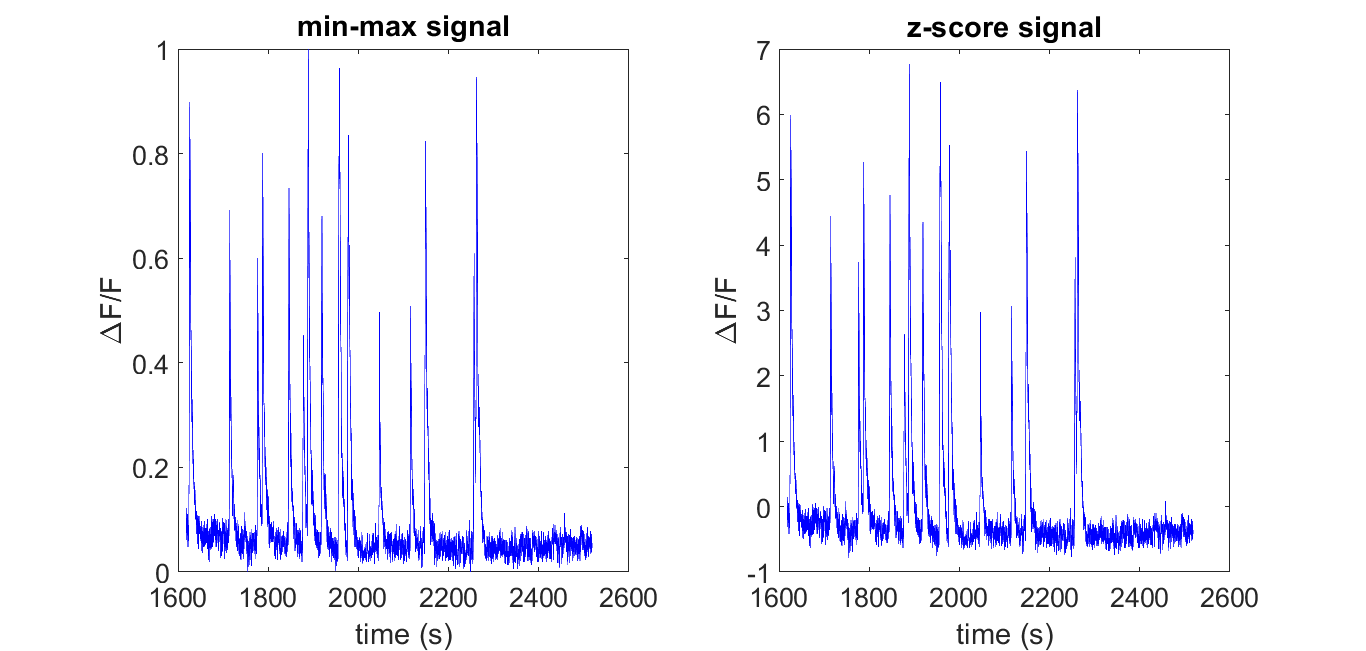
\includegraphics[scale=.4]{normalizations.png} 
		\end{center} 
		\caption{\textit{Different normalizations of the signal. Left: min-max normalization, in which the signal assumes values in $[0,1]$. Right: z-score normalization, with no constraint on the scale of the $y$-axis. }}
		\label{normalizations}
	\end{figure}

The main object of the analysis is given by the calcium signals recorded in every single neurons, expressed in terms of relative fluorescence $\frac{\Delta F}{F}$. Such signals can be subjected to operations and comparisons, either among neurons of a single mouse, or among activities in different mice. based on this scenario, it necesessarily follows that it is fundamental to choose a proper \textit{normalization} of the data which can allow such processes. The literature proposes several ways to treat data, (see Figure \ref{normalizations}):

\begin{enumerate}
	
	\item \textbf{Raw approach}. The raw data, coming from the Inscopix pre-processing described in Section 1.4, are usually not ready to be analyzed yet. Although porcesses of normalizations on the ROI videos, filtering and noise detection  have been already performed, the single information of a fluorescence value $\frac{\Delta F}{F}$ needs to be treated carefully. Every single neuron is characterized by a baseline activity, alternated with rapid and huge spikes. Such baseline value, which biologically represents the \textit{non activity} of a neuron, can take different values across different neurons. Moreover, the values reached by the spikes can appear in different magnitudes across different neurons, but this does not necessarely reflect  what is really happening in the reality: a spike may exhibit smaller amplitudes for the simple fact that less GCaMP protein, which reacts with calcium and show flourescence, was present at that moment, and consequently the spiking of that neuron assumed smaller values. 
	
	\item \textbf{Min-max normalization}. With the min-max normalization, every value $x_t$ of the signal $ x = \left\{ x_t\right\}_{t=1}^N$ at time $t$ is normalized through
	
	\begin{equation}
		x_t^{mm} = \frac{x_t -  \min(x)}{\max(x) - \min(x)}
	\end{equation}
	
	With the min-max normalization, all the signals are bounded in the interval $[0,1]$, where the values $0$ and $1$ occur in correspondence of the lowest and  highest values of the signal, respectively. Therefore, using this normalization, all the signals are treated in the same way, since they are all in the same interval, whatever their original value and scale was in the raw dataset.
	
	\item \textbf{$Z$-score normalization}. For a value  $x_t$ of the signal $ x = \left\{ x_t\right\}_{t=1}^N$, the z-score normalization reads. 
	
	\begin{equation}
	x_t^{z} = \frac{x_t -  \mu}{\sigma}
	\end{equation}
	
	where $\mu$ and $\sigma$ are the mean and standard deviation of the signal, respecitively. The goal of this normalization is to obtain signals with $0$  mean and unitary standard deviation, making them comparable without constrains on their values, as in the case of the min-max normalization. For this reason, $z$-score is the most used type of normalization in the literature.


\end{enumerate}
	
	
	All the different normalizations do not modify the shape of the signals, but their \textit{scale}. As for this work, the choice went on a modificcation on the $z$-score normalization, defined as \textbf{$z$-score on baseline}, in which signals are aligned and then divided by their standard deviations. Therefore, the proposed approach belongs to the $z$-score case, but the alignment is not performed on the mean of each signal, but on their baseline activities. The reason for this is that two signals coming from neurons, when subtracted by their own mean, can still exhibit different baselines. Therefore, with the chosen normalization the alignment is done on such baselines, which are set to $0$ for every neuron, and operations on signals such as sum or direct comparison, can become meaningful.
	
	
	
	\subsection{Behavioural analysis of the task}
	
	
	\begin{figure}[H]
		
		%\begin{center}
		\centering
			
			\hspace*{-1 cm}
			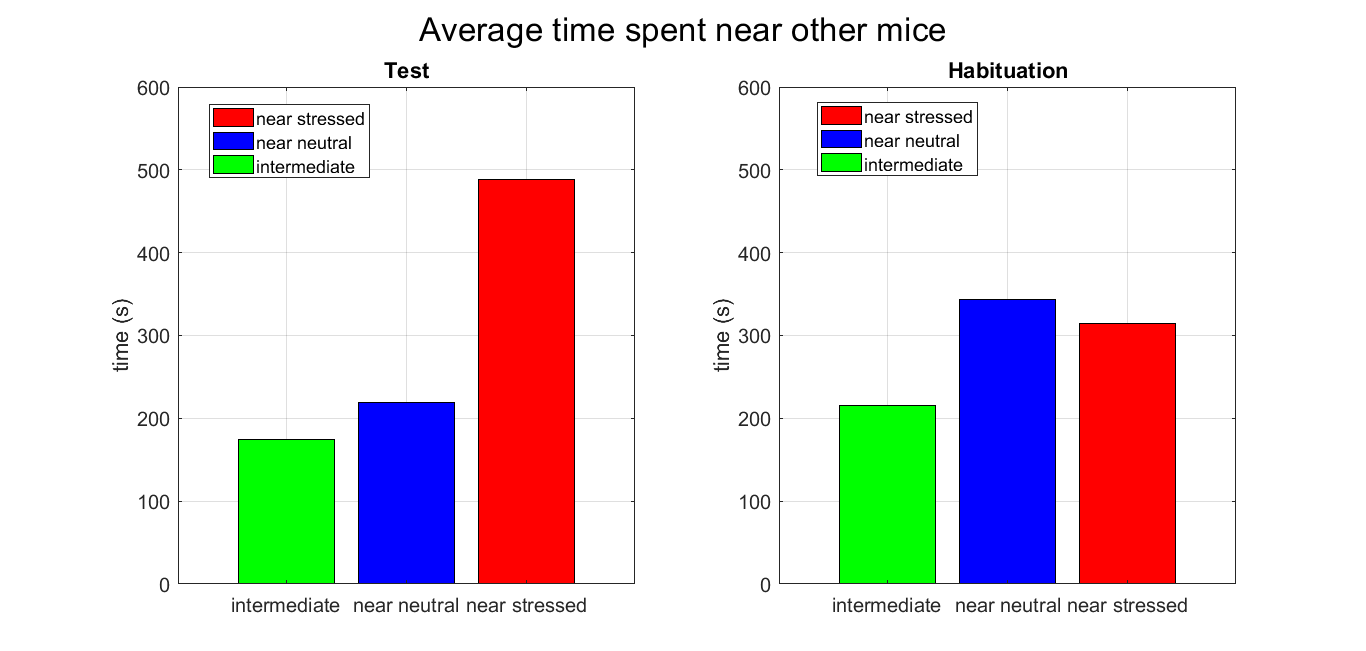
\includegraphics[scale=.37]{times.png} 
		%\end{center} 
		\caption{\textit{Average time spent by the observer near the demonstrator cages, or in the intermediate area. Left: results during the test. Right: results during the habituation. }} \label{times}
		
	\end{figure}
	
In [Scheggia-Managò], the same neuronal population, namely the somatostin interneurons, was observed during a task following a protocol similar to the current emotion discrimination task. In that case, however, the area of interest was the medial prefrontal cortex, and the main focus on the electrophyisiological activity. As results, it was evident that the observer mouse spent more time near the stressed demonstrators, and its neural activity (in terms of action potentials) showed higher values during those periods.\\
In this work, we obtained the following results:

\begin{itemize}
	\item The observer spent a significantly higher time near the stressed demonstrators, rather than near the neutral one or in an intermediate zone (see Figure \ref*{times}). Moreover, in order to rule out the possiblity that this effect was due to spatial factors present in the cage where the stressed mouse was located, a comparison with the habituation has been performed. During the habituation, the observer is free to move in the arena for the same time as in the test, but in the arena the two cages for the demonstrators are empty. The results show clearly that in this situation the observer doesn't show a particular tendency for proximity, and in particular spends considerably less time near the cage of the stressed mouse.
	
	\item In the analysis of the calcium activity, no evidence of correlation between activity  and proximity to demonstrators seemed to emerge during the test: from the recorded neurons, the observer maintains an overall similar average activity through the different areas of the arena. As for the demonstrators, only the neutral appears to show an increase activity during the sniffing with the observer (Figure \ref{activity_barplot}).
	\\
	
	Next, a comparison on the average activity of mice during the phases of the task have been taken into account (see Figure \ref{activities}). The results showed that, in general, the mean activity seems to be higher during the habituation. This happens in particular for the stressed mouse, coherently with the fact that during the habituation, it is  subjected to the stress protocol (forced restrainment), for which it is expected to show higher activity. Overall, the neutral mouse shows smaller values of calcium activity, during both habituation and test, compared to the observer and the stressed conspecifics.
	
\end{itemize}
	
	
		\begin{figure}[H]
		
		\begin{center}
			\hspace*{-1.cm}
			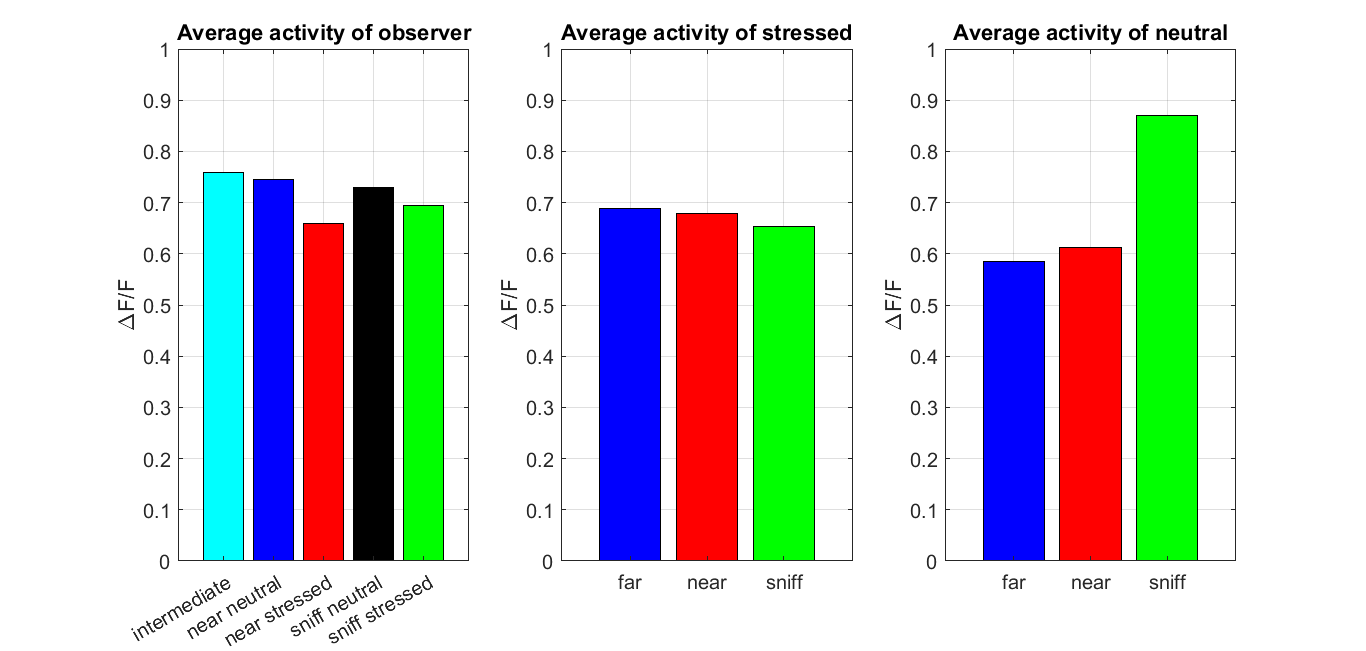
\includegraphics[scale=.35]{activity_barplot.png} 
		\end{center} 
		\caption{\textit{Average activity showed by the mice during the test. Left: observer. No tendencies seem to emerge when it is in intermediate area, close to demonstrators or sniffing with demonstrators. Center: stressed.  Right: neutral.}} \label{activity_barplot}
		
	\end{figure}


\begin{figure}[H]
	
	\begin{center}
	
		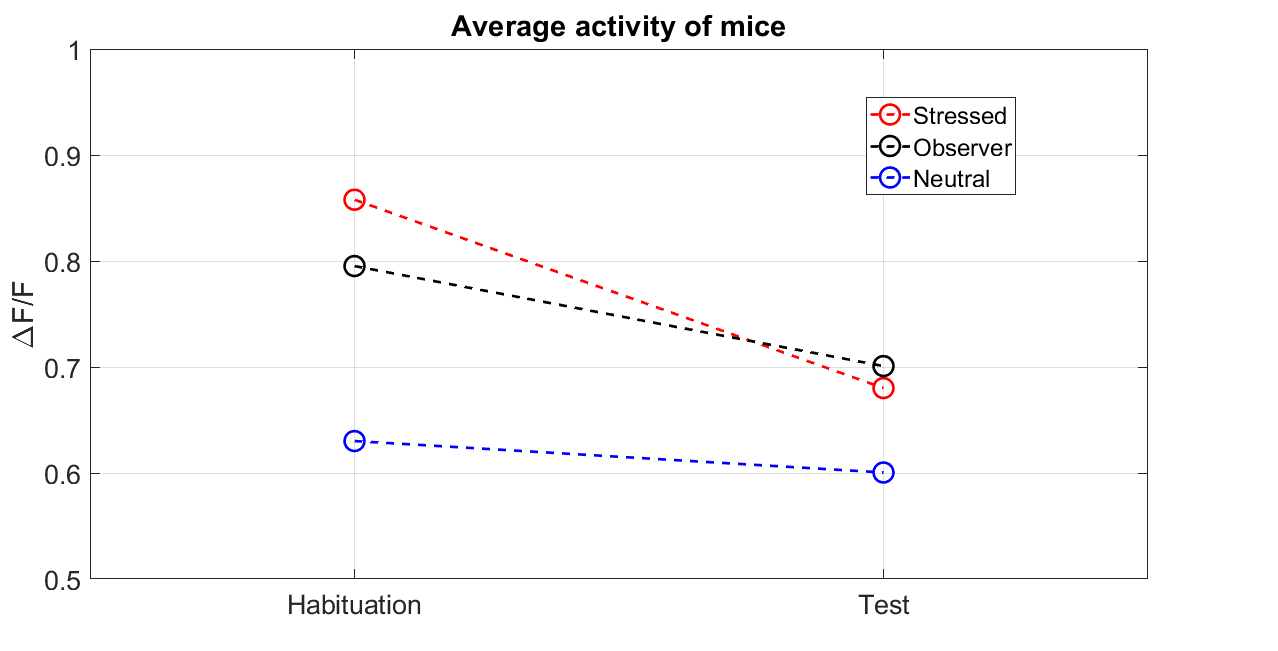
\includegraphics[scale=.35]{activities.png} 
	\end{center} 
	\caption{\textit{Evolution of the average activity of the three mice from the habituation to the test}}
	\label{activities}
\end{figure}


\subsection{Cross-correlation analysis for the mean activity}

\begin{figure}[H]
	
	\begin{center}
		\hspace*{-1.4cm}
		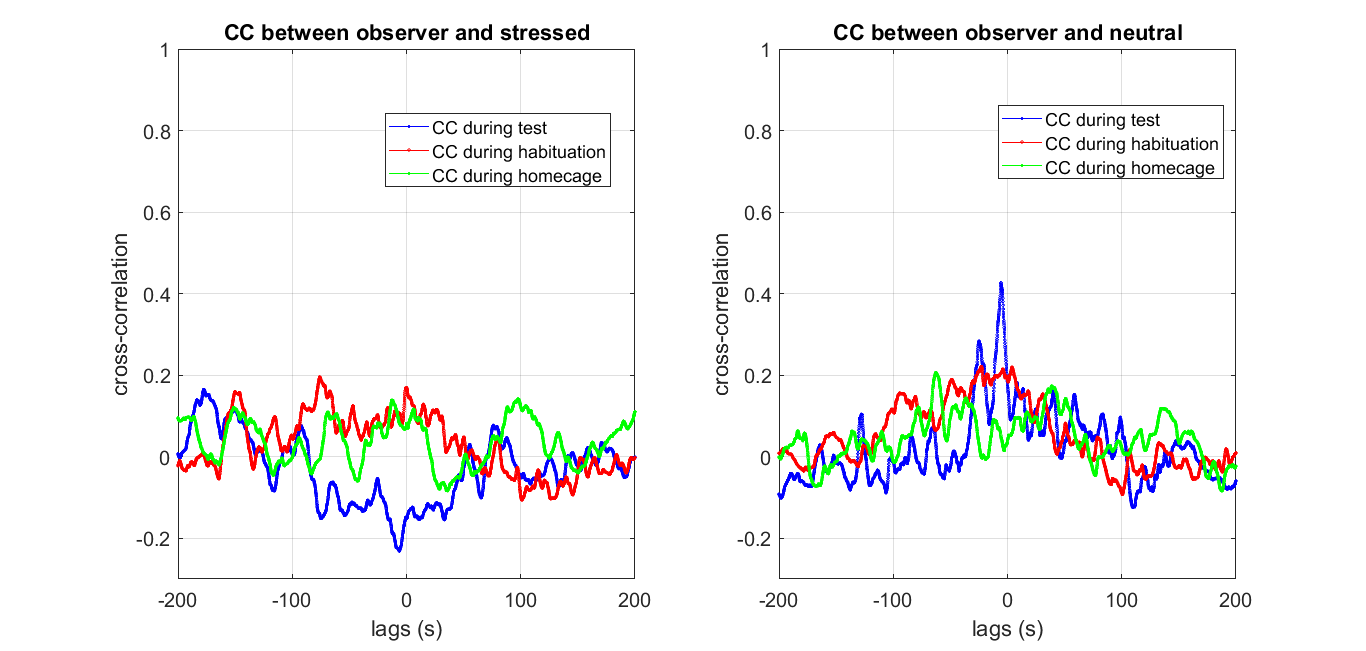
\includegraphics[scale=.4]{average_cc.png} 
	\end{center} 
	\caption{\textit{Left: average cross-correlation between observer and stressed. Right: average cross-correlation between observer and neutral.}} \label{cc}
	
\end{figure}

With the \textit{Interbrain analysis}, we study whether the interactions between two mice are followed by a synchronization of their neural activities. As explained in Section 2.2, one of the main tools for the synchronization analysis is the \textbf{cross-correlation}.\\
As first step, following the approach of [Kingsbury], every mouse has been gifted with its \textit{overall activity}, consisting in a mean of the activities of all its recorded neurons. The spatial data on the position of the observer in the arena during habituation and test, made it possible to divide such mean activities in several parts::

\begin{enumerate}
	\item Restriction to the times of proximity between the observer and the stressed
	\item Restriction to the times of proximity between the observer and the neutral
	\item Restriction to the times of reciprocal sniffing between two mice
\end{enumerate}

The above subdivision allows us to analyze the correlation among the activities of two mice when they are actually close to each other. In this context, a cross-correlation analysis on the mean activity has been performed, comparing what happens during the homecage, habituation and test. During homecage and habituation phases, the three mice are kept separate. Therefore, inspecting the correlation among the activites during these phases is a useful \textit{control}, i.e. a case of comparison in order to see what to expect when correlation should not be present.
\\

After computing the mean of all the $\frac{\Delta F}{F}$ signals in each neuron for every mouse, and applying the above classification $1.-3.$, the cross correlation between observer and stressed and between observer and neutral mean activies has been computed, as described in (ref chap 2). As shown in Figure \ref*{cc}, analyzing the average cross correlation between the two experiments, one can notice the presence of a peak around $ lag=0 $ for the pair observer-neutral in the test phase. This tendency is not present in the control cases of habituation and homecage, making it a proper feature of the test. On the other side, the cross correlation between observer and stressed does not show any particular difference with respect to the homecage and habituation phases. A further verification has been given by observing the cross correlation between the observer and one demonstrator considering the periods when the observer was visiting the opposite demonstrator. As a result, the cross correlation between observer and neutral is inhibited considering the instants when the observer was visiting the stressed, and the cross correlation between observer and stressed remains non significant when the observer is visiting the neutral (Figure \ref{distant}).\\ Overall, these results may show the presence of a synchronization between neural activities of the observer and the neutral demontrsator, but not between the observer and the stressed one, and this effect is present only during the test and during the proximity of the two mice.

\begin{figure}[H]
	
	\begin{center}
		\hspace*{-1.4cm}
		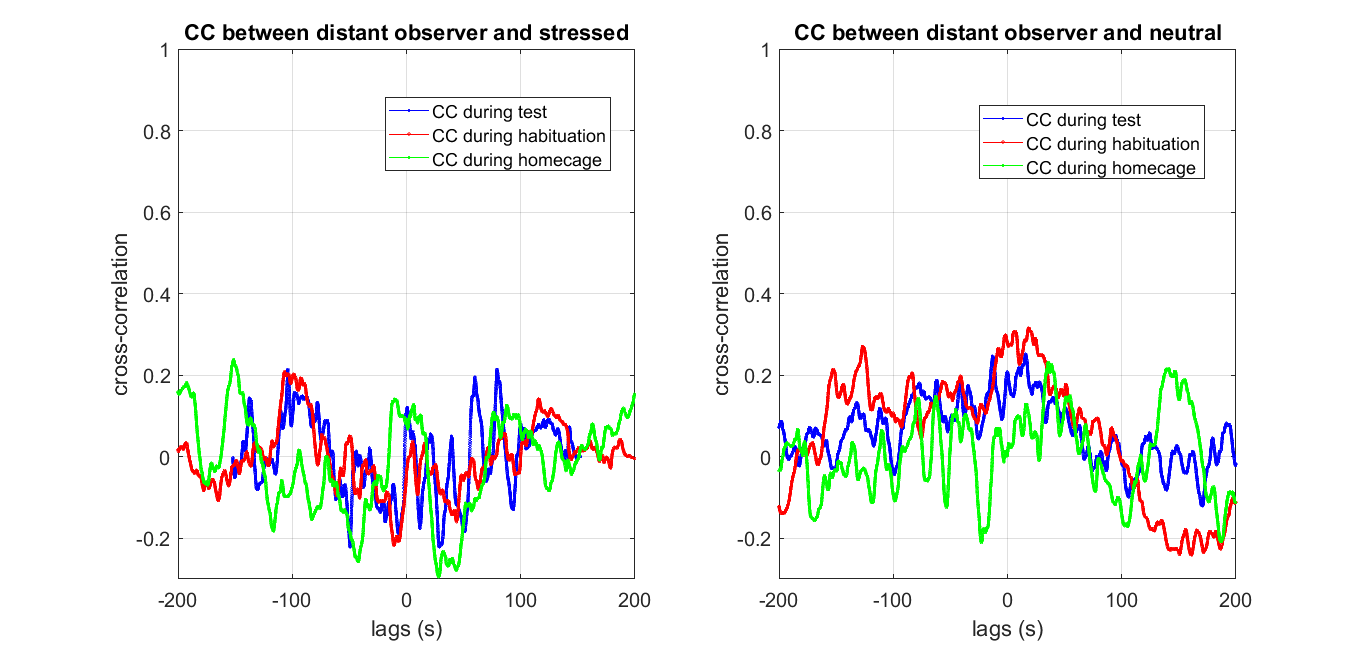
\includegraphics[scale=.4]{cc_distant.png} 
	\end{center} 
	\caption{\textit{Left: average cross-correlation peaks between observer and stressed when the observer is visiting the neutral. Right: average cross-correlation peaks between observer and neutral when the observer is visiting stressed.}} \label{distant}
	
\end{figure}


Next, two particular cases have been considered: the sniffing interactions and the restriction to the first part of test (first 2 minutes of the test). The sniffing is known to be one of the most direct interactions that two mice can display between each other, and therefore is of a particular interest for what could happen at synchronization level. The restriction to the first two minutes of the test is of interest based on previous results [Kingsbury], which show that the first period of interactions among mice is the one which determines some most relevant neural tendencies, such as the display of synchronization.\\
 The obtained results allowed us to draw the following conclusions (Figure \ref{initial}):

\begin{itemize}
	\item Data measurements during the sniffing interactions are coherent with those obtained during the whole test: a peak around $lag=0$ is present only in the cross correlation computed between observer and neutral, but not between observer and stressed
	
	\item Consistent with previous results, the peak of cross-correlation between observer and neutral is higher if we restrict the analysis to the first two minutes of interaction.
	
\end{itemize}

A summary of the cross-correlation results can be seen in Figure \ref{cc_average}. For every case, the values refer to the cross-correlation peak recorded around $lag=0$. While for the observer-stressed case no significant differences arise, between observer and neutral the test phase shows higher correlations, in particular in the sniffing and at the beginning of the test.



\begin{figure}[H]
	
	\begin{center}
		\hspace*{-1.4cm}
		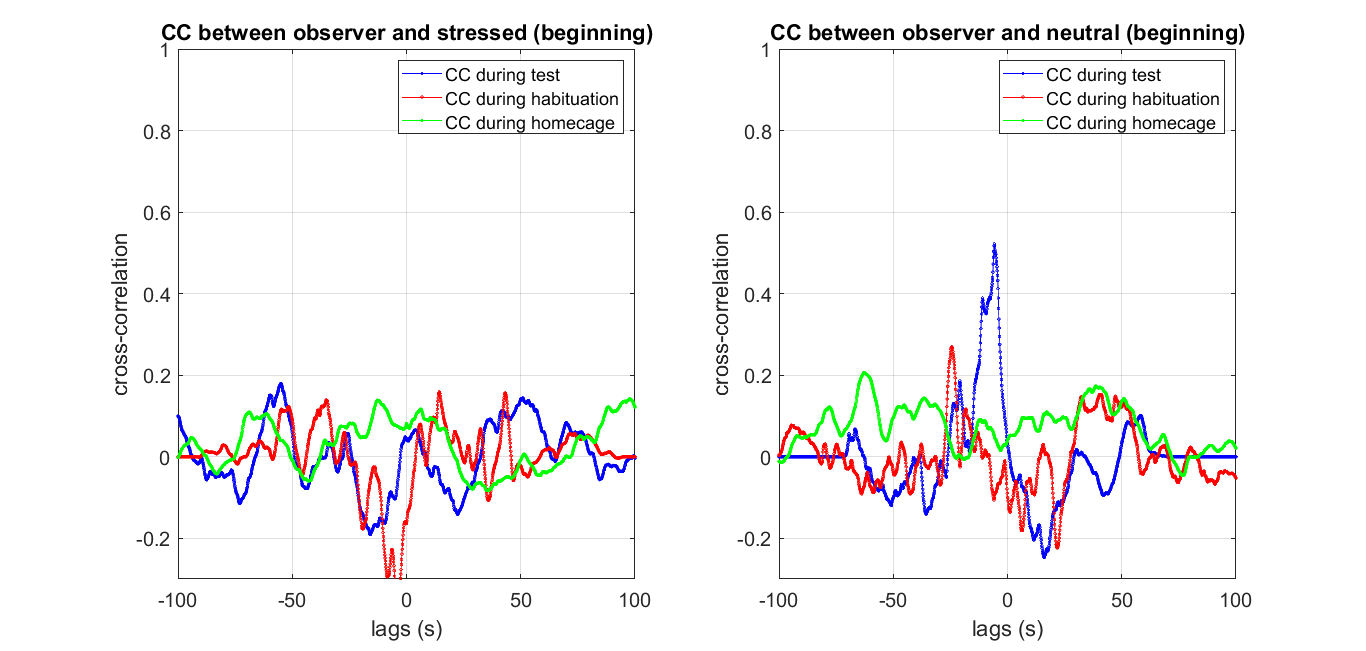
\includegraphics[scale=.4]{average_cc_initial.png} 
	\end{center} 
	\caption{\textit{Left: average cross-correlation between observer and stressed, during the first two minutes of test. Right: average cross-correlation between observer and neutral, during the first two minutes of test.}}
	\label{initial}
\end{figure}

\begin{figure}[H]
	
	\begin{center}
		\hspace*{-1.4cm}
		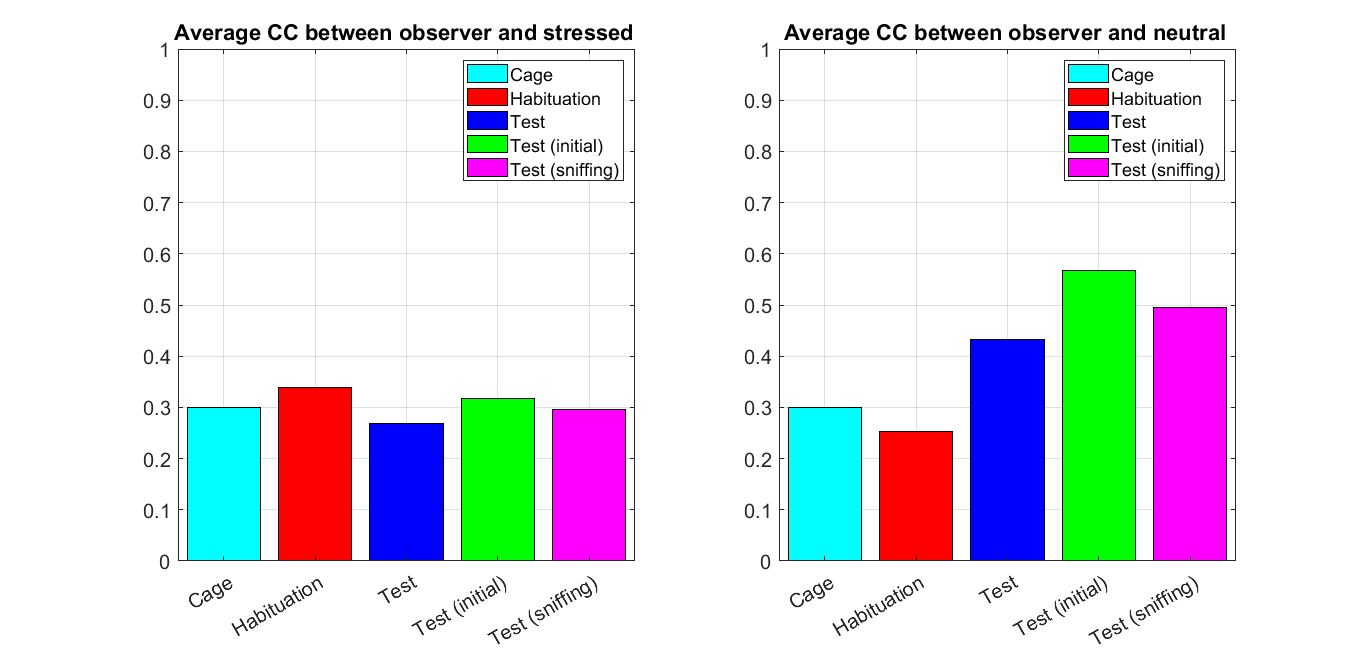
\includegraphics[scale=.4]{cc_average.png} 
	\end{center} 
	\caption{\textit{Left: average cross-correlation peaks between observer and stressed. Right: average cross-correlation peaks between observer and and neutral.}}
	\label{cc_average}
\end{figure}



\subsection{Peak synchronization analysis}

\begin{figure}[H]
	
	\begin{center}
		\hspace*{-1.4cm}
		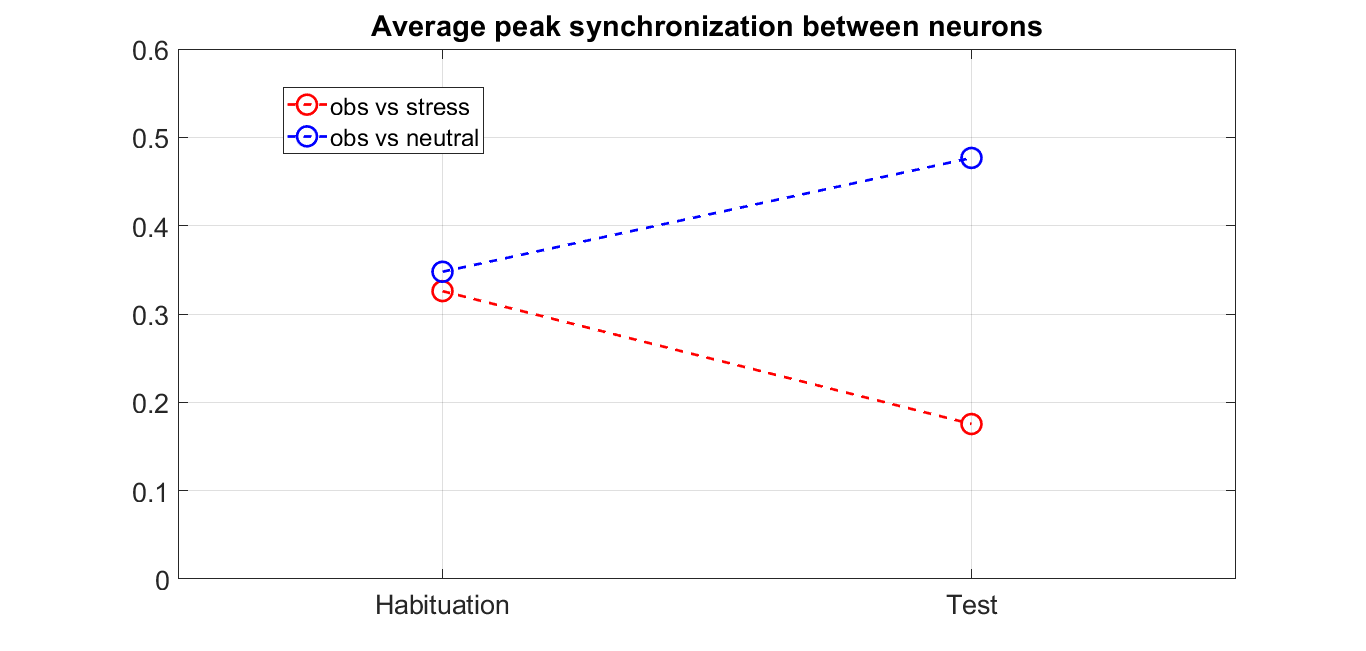
\includegraphics[scale=.4]{avg_pks.png} 
	\end{center} 
	\caption{\textit{Evolution of the average peak synchronization index from the habituation to the test, for the cases observer-stressed and observer-neutral.}} \label{avg_pks}
	
\end{figure}

From the mean activity of the mice, the focus goes now to single neuron synchronization. As presented in Section \ref{section 2.3}, a useful tool to quantify the degree of simultaneous firing between two neurons is given by the \textbf{peak correlation index} \ref{peak index}, which takes into account the number of simultaneous peaks observed during a synchronization time window $dT$ between two signals. As for the present work, the chosen time window, in which two peaks are considered simultaneous, has been set to $dT = 1 s$. The analysis of peak correlation proceeds according the following steps:

\begin{enumerate}
	
	\item Computaton of the peak correlation index for every pair of neurons between the observer and one demonstrator 
	
	\item Computation of the average of the indices for a couple of mice during the test, to be confronted with the same average obtained during the habituation. In this way we can compare the change in simultaneous firing between two neurons from one phase of the task to the other
	
	\item The result on the evolution of the mean correlation index is accompanied by a \textit{one-way ANOVA} test [Book] on the significance of the difference between the two groups of indices. The null hypothesis of the ANOVA states that there is no significance in the difference between the two pupulations, i.e. that $ \mu_1 = \mu_2$,  $\mu_1$  and $ \mu_2$ being the  means of the two populations. Such hypothesis is \textit{rejected} for low $p$-values of the associated test.
	
\end{enumerate}

The obtained results are showed in Figure \ref{avg_pks}. Consistent with the cross-correlation results for the mean activity, the average peak correlation index shows higher values in the test, rather than in the habituation, only for the observer-neutral pair, while for the observer-stressed pair it actually decreases. This average result is consistent between all the two investigated datasets, and in both cases the difference between the indices computed in the test and the ones computed in the habituation is significant ($p$-values of $p = 0.0025$ and $p = 0.0128$ for the two datasets from the ANOVA test)


\subsection{Granger causality analysis}

Granger analysis has been performed in accordance to Section 2.5, to investigate whether the activity of one mouse is Granger-predicting the activity in another. This analysis consists in two statistical tests with null hypothesis
$$ H_0:  Y \hspace{0.2cm} \text{does not G-predicts} \hspace{0.2 cm} X $$
 where in this case $X$ and $Y$ represent the mean activities of the observer and one demonstrator, respectively. In the two analyzed datasets, the results of the tests, in terms of $p$-values, are summarized in Table \ref{Granger table}. Some considerations are in order:

\begin{itemize}
	\item In the first dataset, there is significance to conclude that the observer activity is G-predicting the demontrator ones (both stressed and neutral), while in the second dataset there is evidence only for the prediction from observer to stressed
	
	\item In all cases, it seems that,  when the observer is visiting a demonstrator, the same demonstrator is influenced by the observer, which G-predicts its activity, i.e. the \textit{directionality} of the prediction goes from the observer to the demonstrator
	
	\item The only coherent result is the one involving the stressed demonstrator, whose activity is always G-predicted by the observer one. However, more data should be available in order to draw more definitive conclusions
\end{itemize}



\begin{figure}[H]
	\begin{center}
		\begin{tabular}{ |c|c|c|c| } 
			\hline
			\textbf{Dataset} & \textbf{Directionality} & \textbf{p-value} \\
			\hline
			First & observer $\rightarrow$ stressed & $p = 0.02$ \\ 
			\hline
			First & observer $\rightarrow$ neutral & $p = 0.005$ \\
			\hline
			Second & observer $\rightarrow$ stressed & $p  =  0.01$ \\
		
			\hline
		\end{tabular}
		
	\end{center}
	\caption{Results of the Granger analysis.} \label{Granger table}
\end{figure}



\subsection{Self-experience task}


\begin{figure}[H]
	
	\begin{center}
		\hspace*{-1.4cm}
		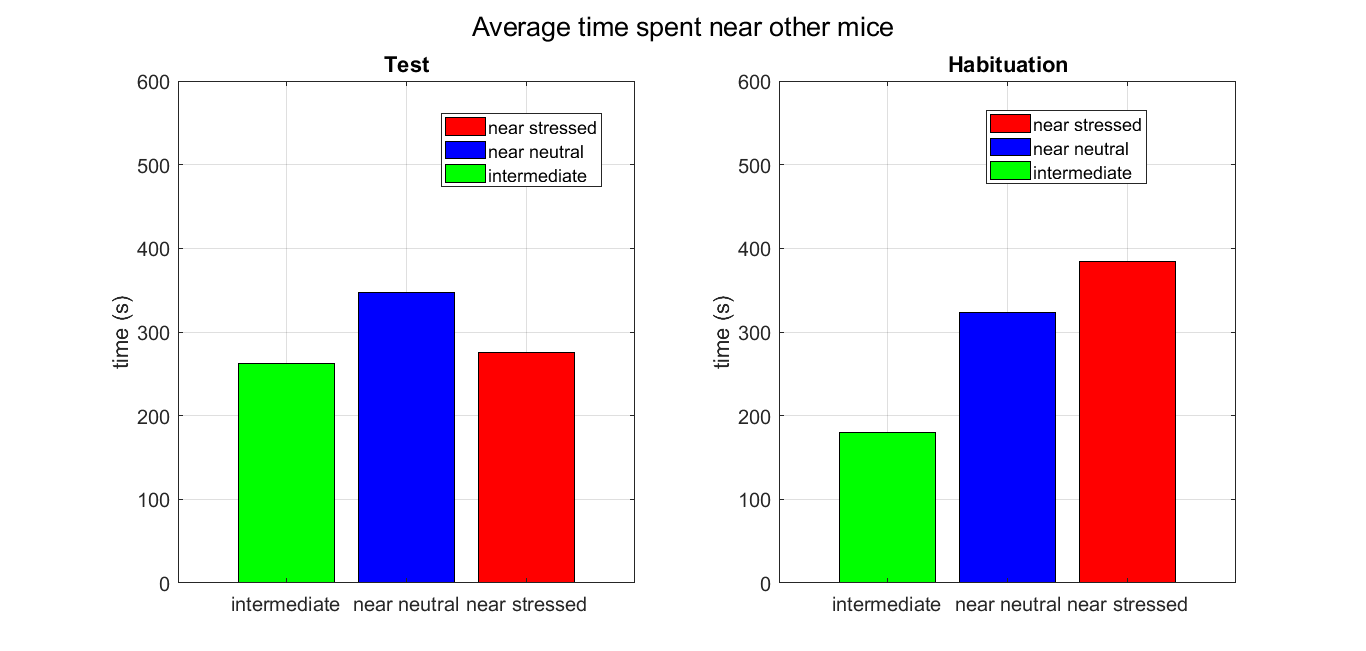
\includegraphics[scale=.4]{times_self.png} 
	\end{center} 
	\caption{\textit{Average time spent by the observer near the demonstrator cages, or in the intermediate area, for the self-experience task. Left: results during the test. Right: results during the habituation.}}
	\label{times_self}
\end{figure}


Two more datasets of the emotion discrimination task have been analyzed. This time, however, they refer to the \textbf{self-experience} configuration, in which the observer has been stressed before the task. The same analyses with the same data normalization as in the standard configuration has been performed. The obtained results are the following:

\begin{itemize}
	\item The observer spends, on average, less time near the stressed, compared to the standard case of non-stressed observer (see Figure \ref{times_self}). This is consistent with an \textit{avoidance} behaviour between two stressed individuals, already observed in past studies [REF?]
	
	\item As for the average activity displayed by the three mice, no relevant differences seem to emerge with respect to the standard case. Once again, the strongest activity is observed during the sniffing between observer and neutral (Figure \ref{activity_barplot_self})
	
	\begin{figure}[H]
		
		\begin{center}
			\hspace*{-1.2cm}
			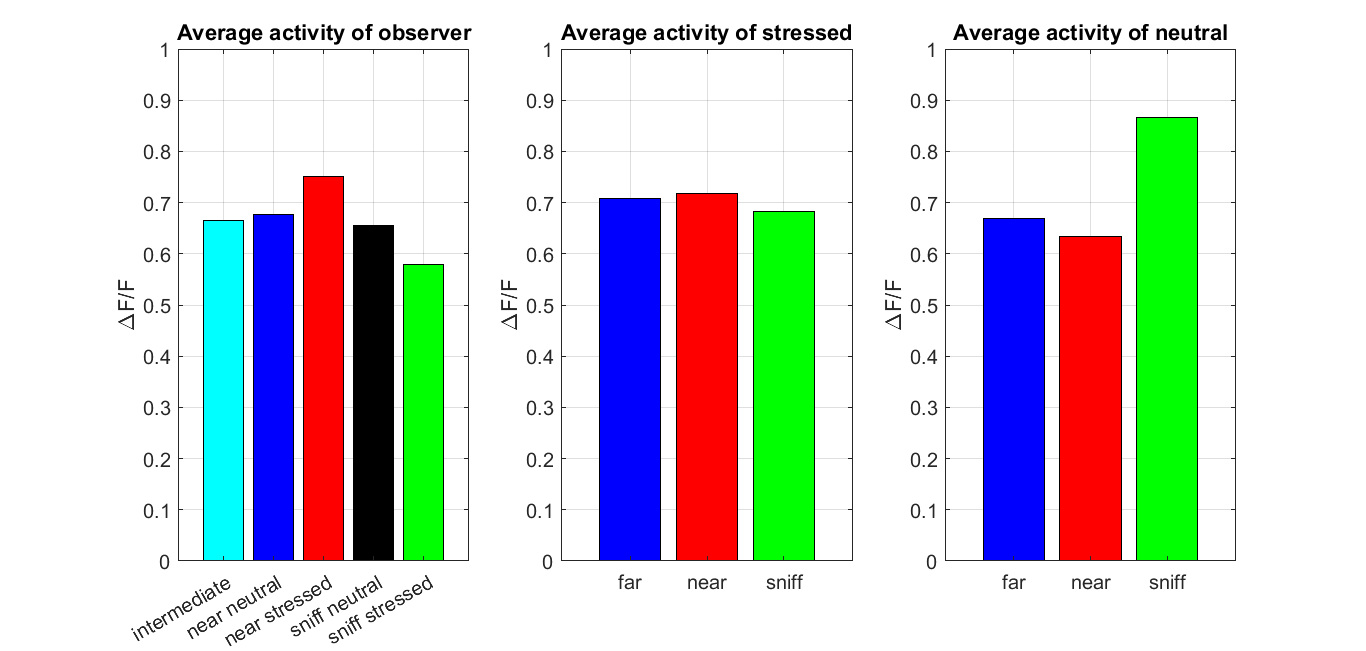
\includegraphics[scale=.38]{activity_barplot_self.png} 
		\end{center} 
		\caption{\textit{Average activity showed by the mice in the self-experience task. Left: observer. Center: stressed. Right: neutral.}}
		\label{activity_barplot_self}
	\end{figure}
	
	\item The cross-correlation peak, observed in the previous case between observer and neutral, now is not present. For both analyzed datasets of self-experience type, no correlation seems to emerge between any pair of mice, not even considering the first two minutes of the task (Figure \ref{average_cc_self})
	
	\begin{figure}[H]
		
		\begin{center}
			\hspace*{-1.4cm}
			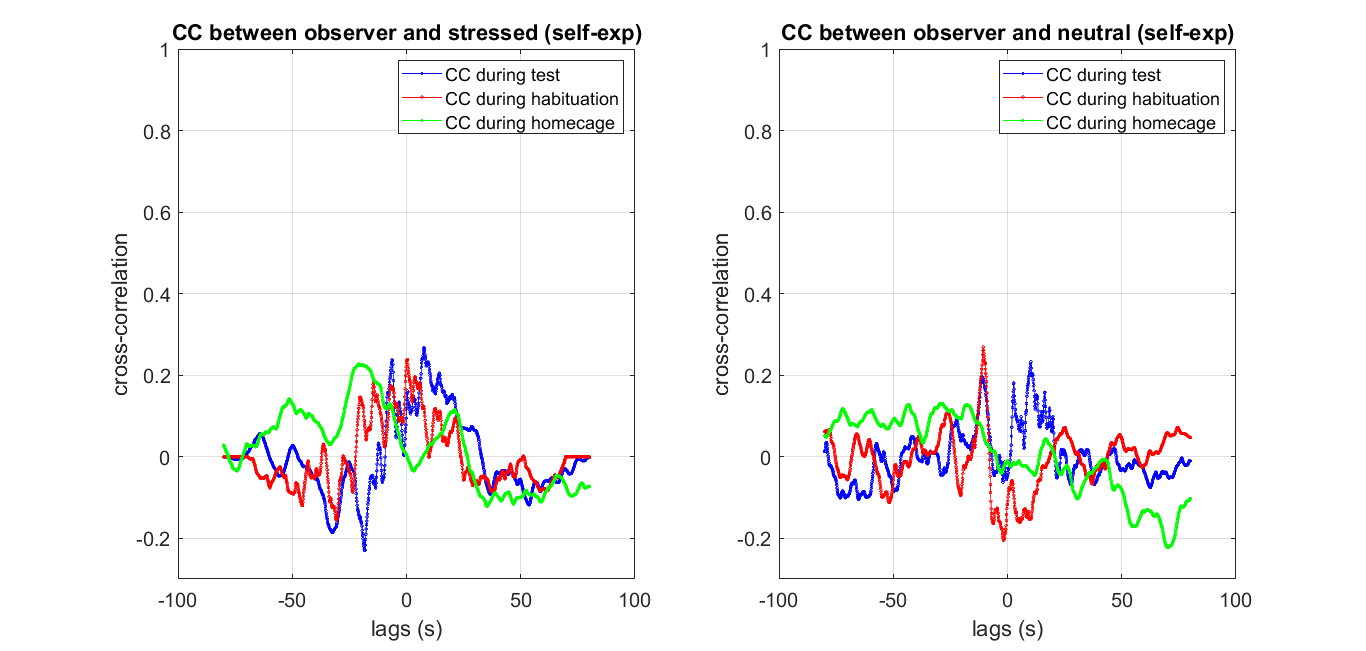
\includegraphics[scale=.4]{average_cc_self.png} 
		\end{center} 
		\caption{\textit{Average cross-correlation, during the first two minutes, in the self-experience task. Left:  between observer and stressed. Right: between observer and neutra.l}}
		\label{average_cc_self}
	\end{figure}
	
	\item The average correlation index slightly decreases in the observer-neutral case and increases in the observer-stressed. These results, however, do not show significance to the ANOVA test (Figure \ref{avg_pks_self})
	
	\begin{figure}[H]
		
		\begin{center}
			\hspace*{-1.4cm}
			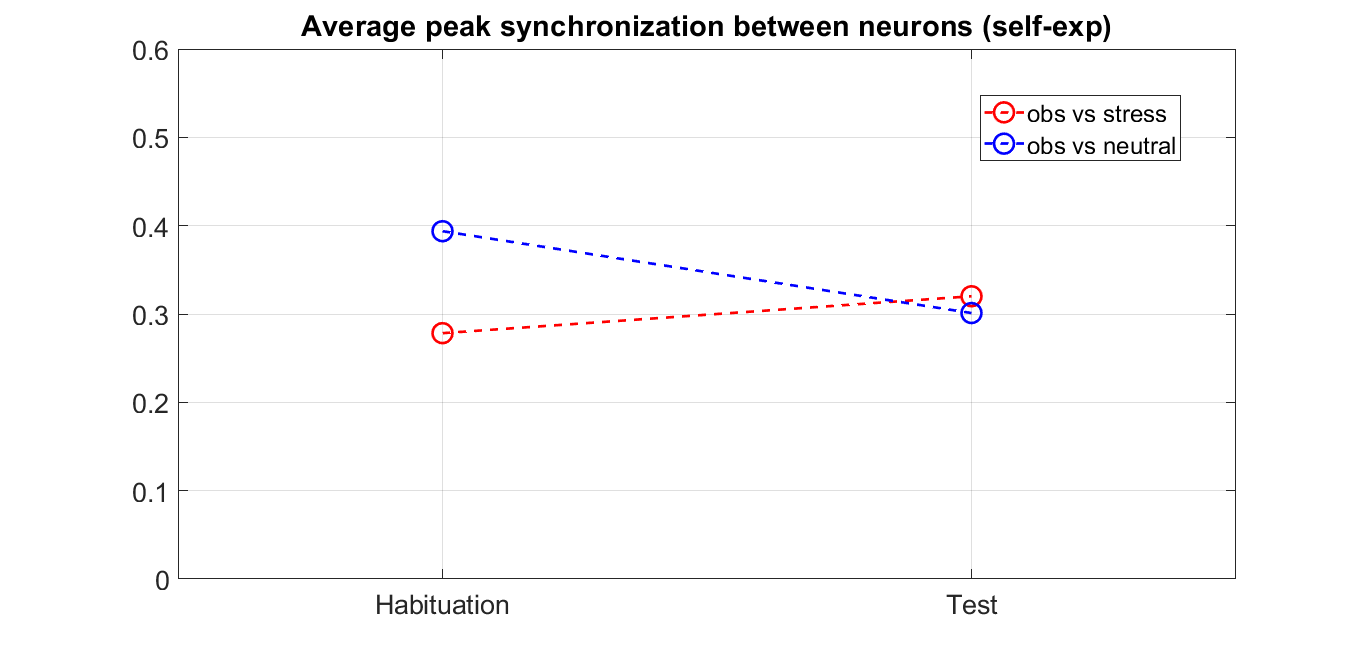
\includegraphics[scale=.4]{avg_pks_self.png} 
		\end{center} 
		\caption{\textit{Evolution of the average peak synchronization index from the habituation to the test, for the  observer-stressed pairs and observer-neutral, in the self-experience task.}}
		\label{avg_pks_self}
	\end{figure}
	
	
	\item Concerning the Granger analysis, in both the analyzed datasets, no significance of Granger prediction in any directionality has been found, both for observer-neutral  for observer-stressed pairs
	
\end{itemize}


\subsection{Conclusions on the emotion discrimination task}


The analyses on the available data (two experiments performed in the standard configuration, two in the self-experience configuration), suggest the manifestation of some unified tendency in the results, and allow us to make some conclusive considerations:

\begin{itemize}
	
	\item The relevant factor explaining the onset or inhibition of the synchronization among neural activities of SOM+ interneurons in the ACC, seems to be the \textit{stress condition}. Indeed, in the standard emotion discrimination task, a higher synchronization of mean neural activities appears between observer and neutral mice, but not observer and stressed, such as in the peak synchronization between neuron pairs. On the other side, when the observer itself is in a stress condition, also the results with the neutral demonstrator are not present, and the other analyses are less significant. This indicates that a stressed mouse may loose the ability to synchronize
	
	\item In order to have credibility, such conclusions need to be repeated in more experiments to be analyzed, since the consistency observed so far only refer to a small dataset
	
	\item In any event, the conclusions do not apply to the whole brain activity of mice. Rather, the conducted analyses consider a very specific neuronal population in a very specific area ( SOM+ neurons in the ACC). It is possible, and actualy plausible, that different areas and different neurons show a different response in activity synchronization
	
\end{itemize}





\end{document}
